\documentclass[11pt]{article}
\usepackage{../../latex/stat4ml_style}

\title{Chapter 6: The EM Algorithm \\ \large Part II --- Introduction to Statistical Learning}
\author{Omid Safarzadeh}
\date{}

\begin{document}
\maketitle

\begin{abstract}
\noindent
Many models have hidden structure --- which cluster a point belongs to, which
mixture component generated it --- that you would need in order to fit the
model, but which you do not observe. Expectation--maximisation breaks that
circle by alternating: guess the hidden assignments softly from the current
parameters (the E-step), then re-estimate the parameters as if those guesses
were data (the M-step). This chapter builds EM on the Gaussian mixture,
proves that each round can only increase the likelihood, and shows the
evidence lower bound that makes the whole thing a single ascent.
\end{abstract}

\tableofcontents

% ======================================================================
\section{Fitting a model with hidden labels}
% ======================================================================

A \keyterm{mixture model} says each observation was drawn from one of $K$
components, but it does not tell you which: with weights $\pi_k$ and component
densities $f_k$, the density of a point is
$p(x) = \sum_{k=1}^K \pi_k\, f_k(x)$. For a \keyterm{Gaussian mixture} each
$f_k$ is $N(\mu_k,\sigma_k^2)$. If we knew each point's component we could fit
each Gaussian from its own points; if we knew the Gaussians we could assign
each point. We know neither --- so EM alternates between soft versions of the
two.

\begin{definition}[The two steps]
The \keyterm{E-step} computes the \emph{responsibility} of component $k$ for
point $x_i$, the posterior probability it came from that component,
\[
  r_{ik} = \frac{\pi_k\, f_k(x_i)}{\sum_{j} \pi_j\, f_j(x_i)}.
\]
The \keyterm{M-step} re-estimates each parameter as a responsibility-weighted
average: $\pi_k = \tfrac1n\sum_i r_{ik}$, $\mu_k = \tfrac{\sum_i r_{ik}x_i}{\sum_i r_{ik}}$,
and similarly for $\sigma_k^2$.
\end{definition}

One iteration is just those two formulas:

\begin{lstlisting}[language=Python]
import math

def gaussian_pdf(x, mu, s2):
    return math.exp(-(x - mu)**2 / (2*s2)) / math.sqrt(2*math.pi*s2)

def em_step(data, pi, mus, s2s):
    K, n = len(pi), len(data)
    R = []                                       # E-step: responsibilities
    for x in data:
        w = [pi[k]*gaussian_pdf(x, mus[k], s2s[k]) for k in range(K)]
        tot = sum(w)
        R.append([wk/tot for wk in w])
    Nk  = [sum(R[i][k] for i in range(n)) for k in range(K)]      # M-step
    pi  = [Nk[k]/n for k in range(K)]
    mus = [sum(R[i][k]*data[i] for i in range(n))/Nk[k] for k in range(K)]
    s2s = [sum(R[i][k]*(data[i]-mus[k])**2 for i in range(n))/Nk[k] for k in range(K)]
    return pi, mus, s2s
\end{lstlisting}

\noindent Run it a few dozen times and the parameters settle; the figure
shows a two-component mixture recovered this way, and --- the point of the
next section --- a log-likelihood that climbs at every step and never falls.

\begin{figure}[h]
  \centering
  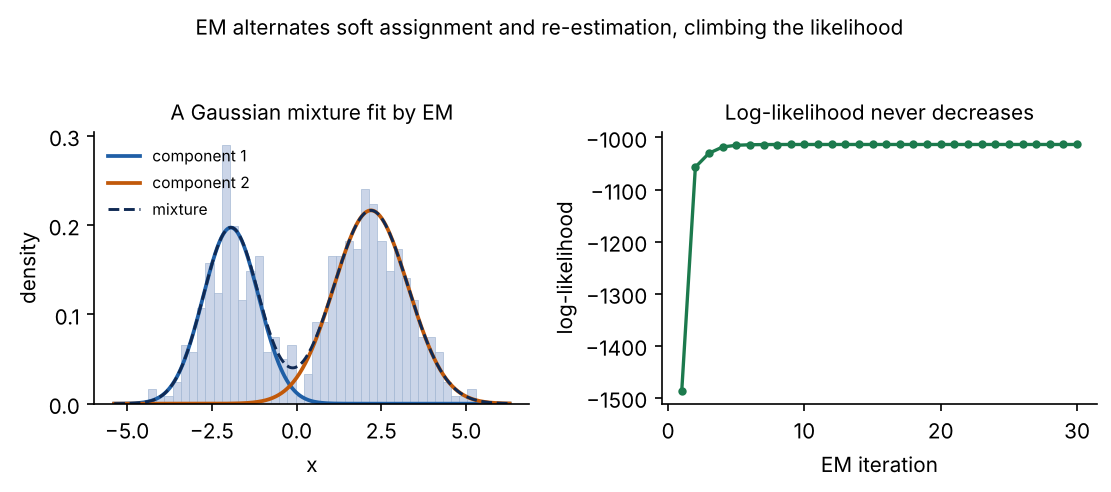
\includegraphics[width=\linewidth]{figures/em_panel.png}
\end{figure}

% ======================================================================
\section{Why the likelihood only goes up}
% ======================================================================

EM optimises the log-likelihood $\log p(x) = \log \sum_z p(x,z)$, where $z$ is
the hidden label, but that sum-inside-a-log is awkward. The trick is to
introduce any distribution $q(z)$ over the hidden labels and split the
log-evidence into two pieces.

\begin{theorem}[Evidence lower bound]
For any distribution $q(z)$,
\[
  \log p(x) = \underbrace{\sum_z q(z)\log\frac{p(x,z)}{q(z)}}_{\text{ELBO}(q)}
            + \underbrace{\sum_z q(z)\log\frac{q(z)}{p(z\mid x)}}_{\mathrm{KL}(q\,\|\,p(z\mid x))}.
\]
Since $\mathrm{KL}\ge 0$ (Jensen's inequality), the ELBO is a lower bound on
$\log p(x)$, tight exactly when $q(z) = p(z\mid x)$.
\end{theorem}
\begin{proof}
Write $p(x,z) = p(z\mid x)\,p(x)$ inside the ELBO:
\[
  \sum_z q\log\frac{p(z\mid x)\,p(x)}{q}
    = \sum_z q\log p(x) + \sum_z q\log\frac{p(z\mid x)}{q}
    = \log p(x) - \mathrm{KL}\big(q\,\|\,p(z\mid x)\big).
\]
Rearranging gives the identity, and $\mathrm{KL}\ge 0$ is Jensen applied to the
concave logarithm.
\end{proof}

Now EM is transparent. The \textbf{E-step} chooses $q(z)=p(z\mid x)$ --- the
responsibilities --- which makes $\mathrm{KL}=0$, so the ELBO rises to meet
$\log p(x)$ exactly. The \textbf{M-step} maximises the ELBO over the
parameters with $q$ fixed, which raises the ELBO further.

\begin{theorem}[Monotone ascent]
Each EM iteration satisfies $\log p(x\,;\theta^{\text{new}}) \ge
\log p(x\,;\theta^{\text{old}})$.
\end{theorem}
\begin{proof}
After the E-step at $\theta^{\text{old}}$ the bound is tight, and the M-step
raises the ELBO while the ELBO remains a lower bound, so
\[
  \log p(x\,;\theta^{\text{new}}) \;\ge\; \mathrm{ELBO}(q,\theta^{\text{new}})
  \;\ge\; \mathrm{ELBO}(q,\theta^{\text{old}}) \;=\; \log p(x\,;\theta^{\text{old}}).
\]
The first inequality is the lower bound, the second is the M-step, and the
final equality is the tightness the E-step created.
\end{proof}

% ======================================================================
\section{EM as coordinate ascent, and what it is cousin to}
% ======================================================================

The two theorems say EM is \keyterm{coordinate ascent} on one objective, the
ELBO $\mathcal{F}(q,\theta)$: the E-step maximises it over $q$, the M-step
over $\theta$, and neither step can decrease it. That is why the likelihood
curve in the figure is monotone --- and also why EM only finds a \emph{local}
optimum: a coordinate ascent stops at the first joint maximum it reaches, so
the result depends on initialisation, and several restarts are standard.

Two neighbours are worth naming. Replace the soft responsibilities with a hard
``winner takes all'' assignment --- $r_{ik}\in\{0,1\}$ --- and fix equal
spherical variances, and EM becomes exactly \keyterm{$k$-means}: the E-step is
``assign each point to its nearest centre'' and the M-step is ``move each
centre to its points' mean'' (Chapter 7). And when $p(z\mid x)$ is itself
intractable, one maximises the ELBO over a restricted family of $q$ instead of
hitting it exactly --- \keyterm{variational inference}, the idea that powers
the variational autoencoder in Part III. EM is the clean special case where
the E-step is exact.

\begin{summarybox}
EM fits models with hidden variables by alternating an E-step --- compute the
responsibilities $r_{ik}=\pi_k f_k(x_i)/\sum_j \pi_j f_j(x_i)$ --- and an
M-step --- re-estimate parameters as responsibility-weighted averages. It
optimises the evidence lower bound, and because
$\log p(x) = \mathrm{ELBO}(q) + \mathrm{KL}(q\|p(z\mid x))$ with
$\mathrm{KL}\ge 0$, each iteration cannot decrease the log-likelihood. EM is
coordinate ascent on the ELBO; its hard-assignment limit is $k$-means and its
approximate-E-step generalisation is variational inference.
\end{summarybox}

\end{document}
